\section{Experimental Evaluation}
To test the effectiveness and efficiency of our model, we design two sets of experiments on both synthetic and real datasets. We evaluate our algorithm on synthetic data because there is not an optimal summarization for real world data. By generating a dataset we are capable of identifying the optimal summarization and in this way test the accuracy and constraints of our model. 

For the synthetic dataset our experiments will answer the following questions: 1. Can the model effectively summarize event sequences? 2. Is the model efficiently performing the summarization? 3. Can we obtain a similar cost for the model by performing random cuts and clusters in the dataset? For the real world dataset our experiments will answer the following questions: 1. The model finds useful patterns from the real world dataset? 2. The summarization is easy to understand?

\subsection{Synthetic Data}
In order to evaluate the proposed   algorithms, we shall compare its output on the synthetic data with the model used to generate the data in the first place. We know the exact cuts (and thereby the induced segments) in the timeline and the grouping of the events in each segment. With this we can define  the ideal (or optimal) output for our algorithm. We will evaluate the algorithms over multiple generated datasets. Table \ref{tab:expNotation} shows the notation used in the rest of the section to describe the experiments.

\begin{table}[!h]
\centering
    \caption{Experiments Notation}     
    \label{tab:expNotation}
    \begin{small}
    \begin{tabular}{|ll|}
    \hline
    {\bfseries Symbol} & {\bfseries  Description}      \\
    \hline
    $n$ & length of timeline  \\    \hline
     $m$ & number of event types  \\    \hline
     $s$ & number of segments  \\    \hline
      $p$ & number of correlation patterns  \\    \hline
       $d_n$ & degree of noise \\    \hline
        $e$ & number of events in one pattern  \\    \hline
    \end{tabular}
    \end{small} 
\end{table}

We create 6 datasets (that we call $M_1, ..., M_6$) by fixing $n=250$, $m=150$, $s=10$, $p=30$, $e=50$. We change the noise from 0 to 0.5 incrementing by 0.1. This means that to introduce 0.1  noise  to our initial dataset, each value of the set, with a probability of $10\%$, will be changed for a random number given by a Poisson distribution with a rate parameter of $\lambda=5$. In each dataset 30 correlation patterns with 30 defined segments in the timeline are created with 50 events in each pattern. Each dataset is randomly ordered before executing the summarization algorithm.

Table \ref{tab:syn1000} show the results of how many segments and clusters of events are found. For a pattern to be considered found, every event from the initial setup should be in it. Our model finds correct cuts and clusters in a dataset with 0.4\% of added noise.

\begin{table}[!h]
\centering
    \caption{Summarization accuracy for synthetic dataset, $n=250$, $m=150$, $p=20$, $c=50$, $e=50$}     
    \label{tab:syn1000}
    \begin{small}
    \begin{tabular}{|l|l|l|l|}
    \hline
    {\bfseries Model} &{\bfseries $d_n$} & {\bfseries  No. Segments} &  {\bfseries  No. Patterns}     \\
    \hline
    $M_1$&$0$ &  10/10 & 30/30\\    \hline
     $M_2$&$0.1$ & 10/10  & 30/30\\    \hline
     $M_3$& $0.2$ & 10/10 & 30/30\\    \hline
     $M_4$  &$0.3$ & 10/10 & 30/30\\    \hline
     $M_5$  & $0.4$ & 10/10  & 30/30\\    \hline
     $M_6$  & $0.5$ & 6/10 & 16/30\\    \hline
    \end{tabular}
    \end{small} 
\end{table}

We will evaluate the quality of the solution produced by our algorithm by using the compression ratio, CR, defined in \cite{Kiernan:constructing}.
\textbf{Compression Ratio:} or $CR(A)$, given algorithm $A$  is equal to the optimal total length of the data compressed with algorithm $A$ divided by encoding the data set $D$ as it is. In our case this means a model with $n$ cuts in the timeline and $m$ groups per segment. The formula is defined as,
$$CR(A)=\frac{TL(A)}{TL(D)}.$$

Figure \ref{fig:noise} shows that for each of the models in Table \ref{tab:syn1000}, when the percentage of noise increases the CR value increases too. This shows that our model gives a lower cost when patterns are present. Figure \ref{fig:random} shows this effect too. The red dot shows the optimal model value for each dataset, positioning the dot far from the best cost generated from random cuts. For the noiseless dataset the optimal code-length is far from the minimum cost model generated randomly. For the other datasets it shows that our model benefits if more patterns exists, giving a lower optimal cost for the encoded dataset. To investigate the effect of the number of patterns in a dataset, we create 7 datasets by fixing $n=50$, $m=150$, $s=2$, $e=25$. We change the percentage of patterns $p$ from 0.1 to 0.7 incrementing by 0.1. Figure \ref{fig:pattern} shows that when the percentage of patterns increase in a dataset the compression ratio value decreases.

\begin{figure}
\begin{minipage}[c]{0.4\linewidth}
%\begin{figure}
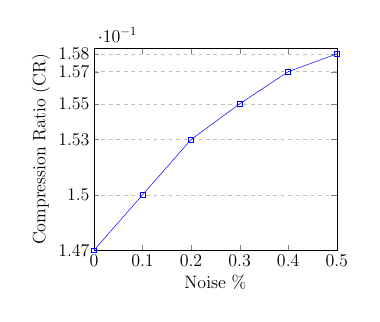
\begin{tikzpicture}[scale=0.45]
\begin{axis}[
    %title={Temperature dependence of CuSO$_4\cdot$5H$_2$O solubility},
    xlabel={Noise \%},
    ylabel={Compression Ratio (CR)},
    xmin=0, xmax=0.5, 
    ymin=0.1467, ymax=0.158, scaled y ticks={base 10:1},
    xtick={0,0.1,0.2,0.3,0.4,0.5},
    ytick={0.1467,0.1498,0.1529,0.1549,0.1567,0.1577},
     label style={font=\Large},
    tick label style={font=\Large},
    %legend pos=north west,
    ymajorgrids=true,
    grid style=dashed,
]
 
\addplot[
    color=blue,
    mark=square,
    ]
    coordinates {
    (0,0.1467)(0.1,0.1498)(0.2,0.1529)(0.3,0.1549)(0.4,0.1567)(0.5,0.1577)
    };
    %\legend{c}
\end{axis}
\end{tikzpicture}
\caption{When the noise increases, the compression ratio increases. Lower value of CR is preferred.} \label{fig:crnoise}
%\end{figure}
\label{fig:noise}
\end{minipage}
\hfill
\begin{minipage}[c]{0.4\linewidth}
%\begin{figure}
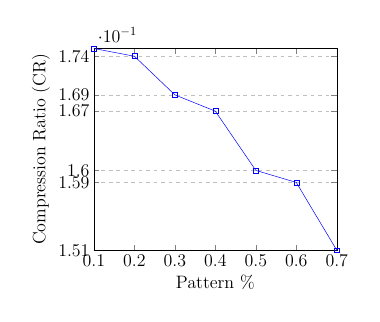
\begin{tikzpicture}[scale=0.45]
\begin{axis}[
    %title={Temperature dependence of CuSO$_4\cdot$5H$_2$O solubility},
    xlabel={Pattern \%},
    ylabel={Compression Ratio (CR)},
    xmin=0.1, xmax=0.7, 
    ymin=0.1510, ymax=0.1745, scaled y ticks={base 10:1},
    xtick={0.1,0.2,0.3,0.4,0.5,0.6,0.7},
    ytick={0.1736,0.1691,0.1672,0.1603,0.1589,0.1510},
    label style={font=\Large},
    tick label style={font=\Large},
    %legend pos=north west,
    ymajorgrids=true,
    grid style=dashed,
]
 
\addplot[
    color=blue,
    mark=square,
    ]
    coordinates {
    (0.1,0.1745)(0.2,0.1736)(0.3,0.1691)(0.4,0.1672)(0.5,0.1603)(0.6,0.1589)(0.7,0.1510)
    };
    %\legend{c}
\end{axis}
\end{tikzpicture}
\caption{When number of patterns increase, the compression ratio decreases. n=50, m=150, e=25} \label{fig:addpatterns}
%\end{figure}
\label{fig:pattern}
\end{minipage}%
\end{figure}  


\begin{figure}[h!]
\begin{minipage}[t]{0.22\textwidth}
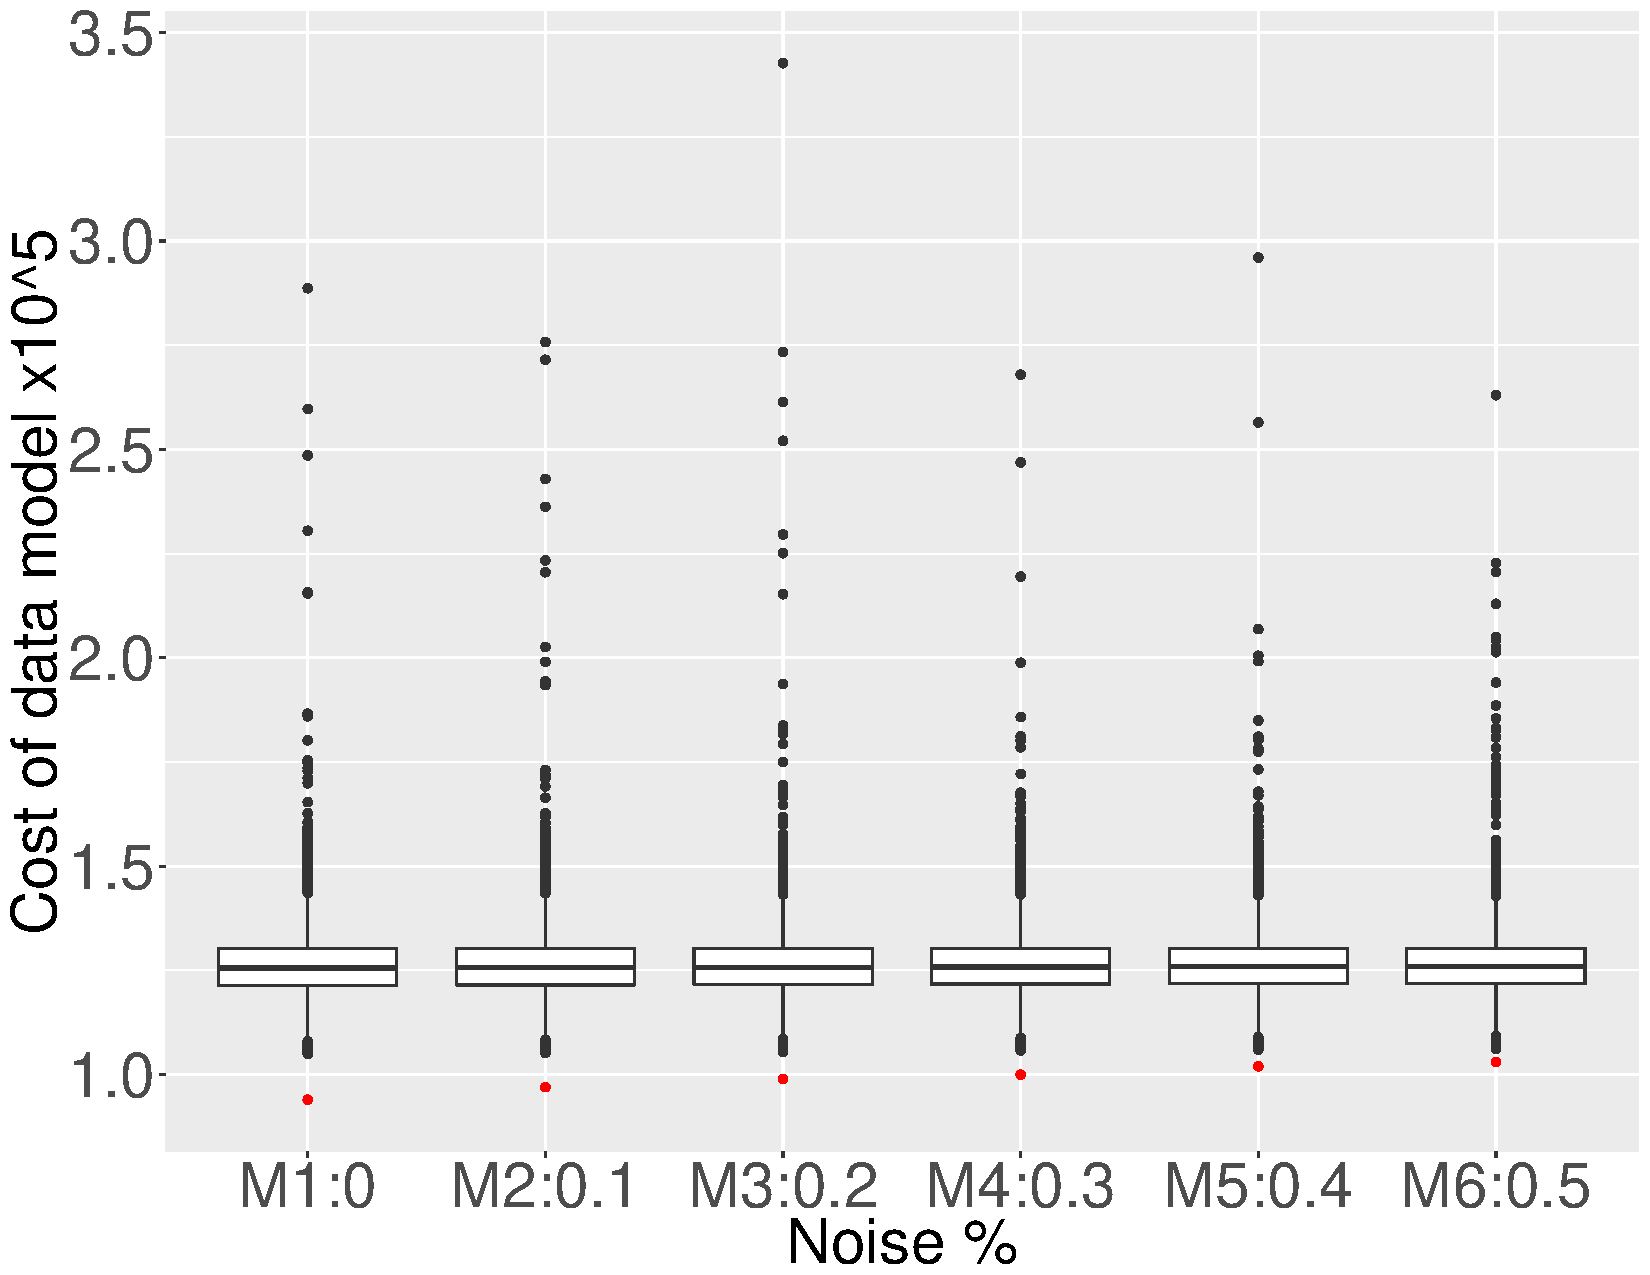
\includegraphics[width=\linewidth,keepaspectratio=true]{images/random.pdf}
   \caption{For each model in Table \ref{tab:syn1000} we generated 100,000 random models with a random assignment of cuts for segments and local clusters. Red dots represents the optimal code length for each dataset found by our optimization algorithm.}
    \label{fig:random}
\end{minipage}
\hspace*{\fill}
\begin{minipage}[t]{0.23\textwidth}
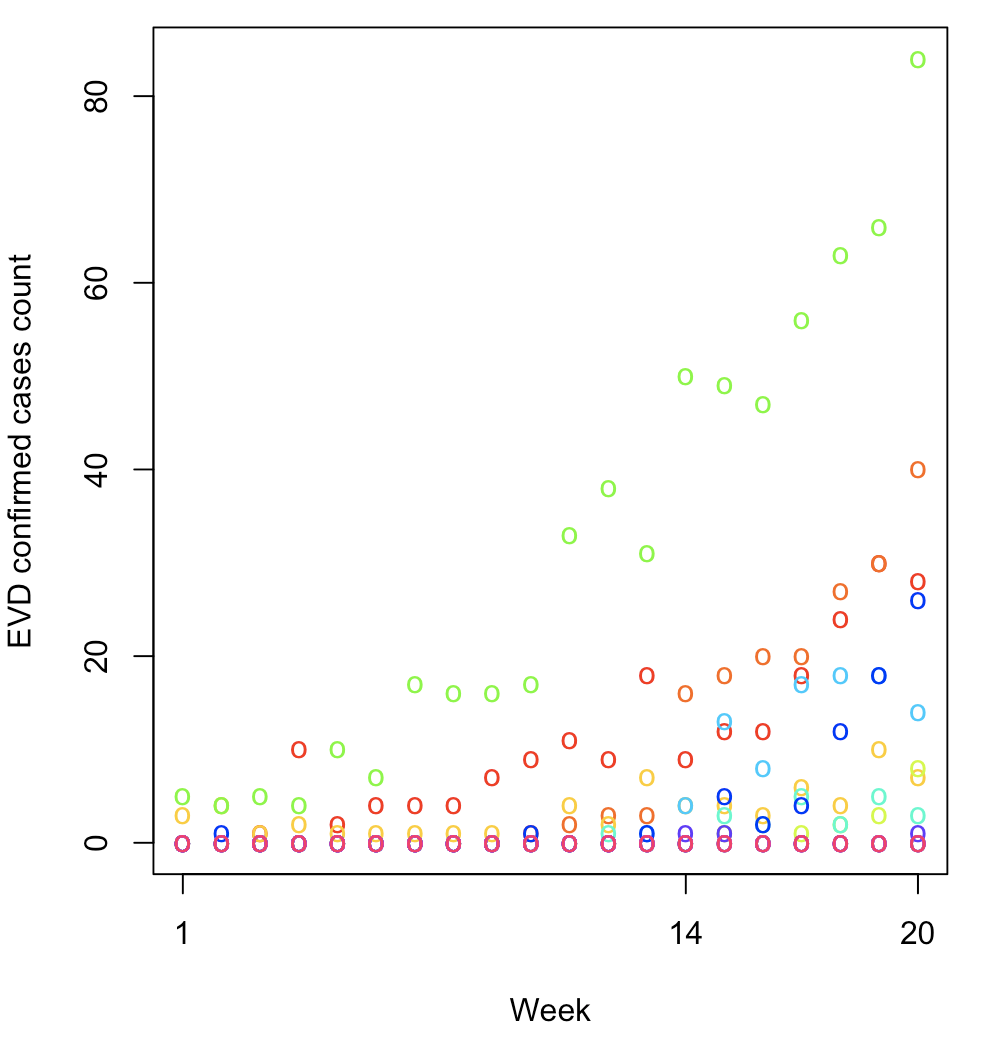
\includegraphics[width=\linewidth,keepaspectratio=true]{images/ebola.pdf}
   \caption{Recorded weekly cases of Ebola infections for 15 counties in Liberia. Here, each county is a colored event sequence. The algorithm segments  the time on week 13 and the local clusters, presented in Table \ref{tab:ebola}, tell a story consistent with the analysis made by experts in the field of epidemiology. 
}
  \label{fig:ebola}
\end{minipage}
\end{figure}  

\subsection{Real Data}
\label{sec:realdata}
\subsubsection{Summarization of Ebola Virus Disease cases}
We analyze data from an agent-based model framework developed for forecasting the 2014-2015 Ebola epidemic in Liberia \cite{VENKATRAMANAN:2018}. We have the recorded weekly cases of Ebola infections for the 15 counties in Liberia. Figure \ref{fig:ebola} shows the cases and each county is a colored event sequence. The algorithm segments  the time on week 13 and the local clusters, presented in Table \ref{tab:ebola}, tell the following story consistent with the analysis made by experts in the field of epidemiology. For the first 13 weeks Grand Cape Mount is on it's own cluster with 203 cases. The second cluster groups Bomi and Gbarpolu with the highest counts with 79 and 28. cases. The rest of counties are clustered with 9 to 0 cases for the 13 weeks. The segmentation of week 13 is important because certain practices were enforced after that week. Traditional burial practices were observed among all communities which involves washing/touching/kissing the bodies during ceremony. The practices are confirmed to contribute to the spreading of Ebola Virus Disease (EVD). No effective safe burial protocol has been enforced till week 13. Also, no contact tracing cases were followed till week 13 and no Ebola Treatment Unit (ETU) were opened till week 13. 
 
From Table \ref{tab:ebola} it is easy to see that cases are high through the 20 weeks in Grand Cape Mount and Bomi. But Gbarpolu, from having a high number of cases from week 1 to 13, descends to a low level cluster 4 in week 14.
 
\begin{table}[!h]
\centering
    \caption{Summarization of Ebola virus disease confirmed cases in Liberia, 2015.}     
    \label{tab:ebola}
    \begin{small}
\begin{tabular}{p{0.35in}p{0.3in}p{2.3in}}
    \hline
    {\bfseries Segment} &{\bfseries Weeks} & {\bfseries  Clusters}   \\
    \hline
    1&1-13&  {\bfseries 1:} Grand Cape Mount    \\
    & & {\bfseries 2:}  Gbarpolu, Bomi   \\
    & & {\bfseries 3:} Bong, Montserrado, Lofa, Margibi, Grand Bassa, Grand Gedeh, Grand Kru, Maryland, Nimba, River Gee, Rivercess, Sinoe\\    \hline
     2&14-20 & {\bfseries 1:} Grand Cape Mount   \\
     & & {\bfseries 2:}  Bong, Bomi   \\
     & & {\bfseries 3:}  Margibi, Montserrado   \\
     & & {\bfseries 4:}  Gbarpolu, Lofa, Grand Bassa   \\
     & & {\bfseries 5:}  Nimba,Grand Gedeh, Grand Kru, Maryland, River Gee, Rivercess, Sinoe\\    \hline
    \end{tabular}
    \end{small} 
\end{table}

\subsubsection{Summarization of Global Landslides}
The Global Landslide Catalog (GLC) was developed with the goal of identifying rainfall-triggered landslide events around the world. The GLC considers all types of mass movements triggered by rainfall, which have been reported in the media, disaster databases, scientific reports, or other sources and has been compiled since 2007 at NASA Goddard Space Flight Center \cite{Kirschbaum:2010}. 
From the GLC, we analyze almost ten years (from 01/01/2007 to 10/25/2016) of reports of fatalities by landslides. 
%Figure \ref{fig:fatalities} shows the event sequences of fatalities by landslides for $m=102$ countries in $n=3586$ days; we can see how it's not trivial to define patterns and important segments in time from the plot. 
For this dataset the summarization outputs 9 segments and the corresponding local clusters are detailed in Table \ref{tab:landslide}.

%\begin{figure}[!tbh] 
 % \begin{center}
  %     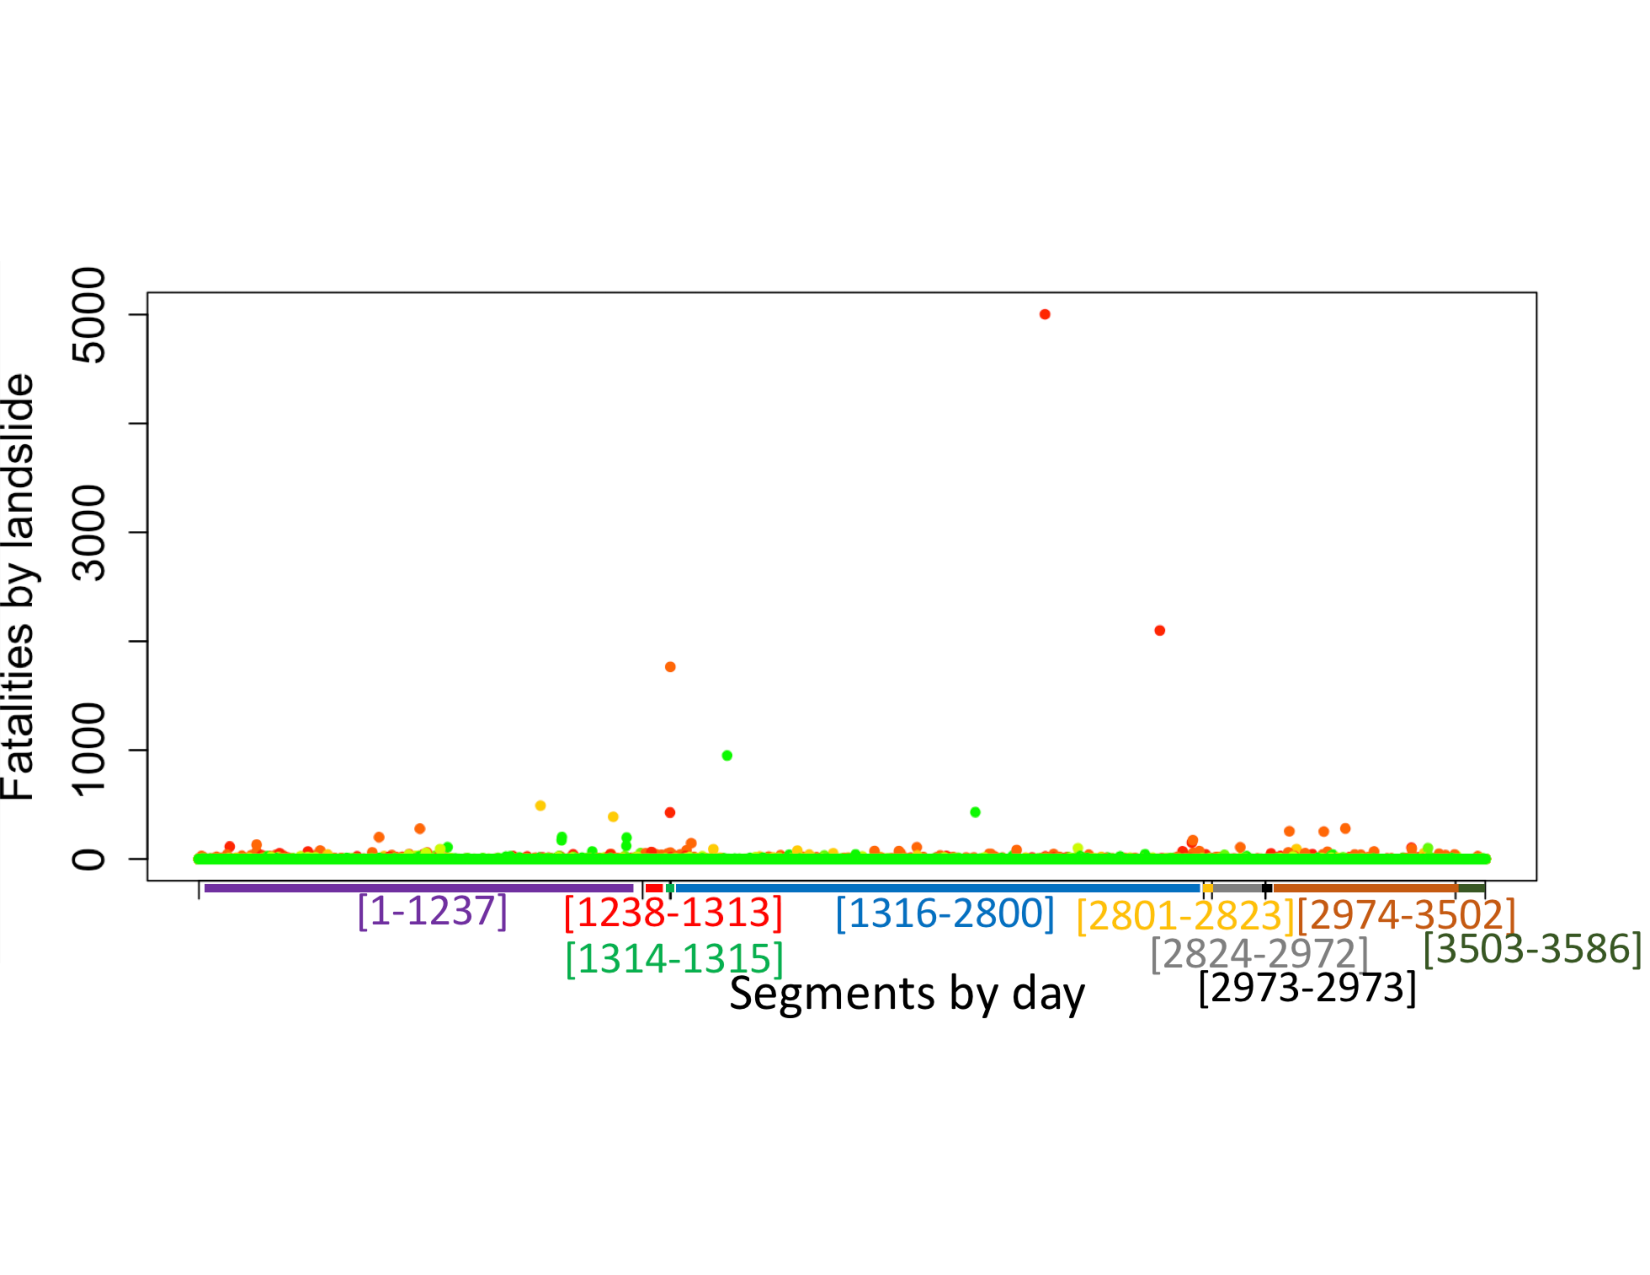
\includegraphics[trim = 0in 1.7in 0in 1.8in, clip,scale=0.35]{images/landslide.pdf}
 % \end{center}
 %  \caption{Reports of landslides fatalities occurrences from 01/01/2007 to 10/25/2016 (3586 days), from the Global Landslide Catalog (GLC). Our model summarizes the dataset providing 9 %segments in time (represented in the Figure with different colors) and local clusters detailed in Table \ref{tab:landslide}.
%}
%  \label{fig:fatalities}
%\end{figure}


\begin{table}[!h]
\centering
    \caption{Summarization of Fatalities by landslides from the Global Landslide Catalog, from 01/01/2007 to 10/25/2016.}     
    \label{tab:landslide}
    \begin{small}
\begin{tabular}{p{0.35in}p{0.55in}p{0.6in}p{1.2in}}
    \hline
    {\bfseries Segment} &{\bfseries Begin Day} &{\bfseries Begin Date} & {\bfseries  Clusters}   \\
   &{\bfseries End Day} &{\bfseries End Date} &  \\
    \hline
    1&1 & 01/01/2007&{\bfseries 1:} All countries    \\
      &1237& 05/21/2010&   \\
    \hline
        2&1238 & 05/22/2010&{\bfseries 1:} China   \\
      &1313& 08/05/2010&  {\bfseries 2:} All other countries    \\
    \hline
        3&1314 & 08/06/2010&{\bfseries 1:} China   \\
      &1315& 08/07/2010&  {\bfseries 2:} India    \\
       && &  {\bfseries 3:} Pakistan    \\
       && &  {\bfseries 4:} All other countries     \\
    \hline
            4& 1316 & 08/08/2010&{\bfseries 1:} All countries   \\
      & 2800 & 08/31/2014&     \\
     \hline
      5& 2801 & 09/01/2014&{\bfseries 1:} India   \\
      & 2823 & 09/23/2014&  {\bfseries 2:} China, Pakistan  \\
      &  & &  {\bfseries 3:} All other countries  \\
     \hline
       6& 2824 & 09/24/2014&{\bfseries 1:} All countries   \\
      & 2972 & 02/19/2015&   \\
     \hline
        7& 2973 & 02/20/2015&{\bfseries 1:} All countries   \\
      & 2973 & 02/20/2015&   \\
      &  & &  \\
     \hline
        8& 2974 & 02/21/2015&{\bfseries 1:} All countries   \\
      & 3502 & 08/02/2016&   \\
     \hline
      9& 3503 & 08/03/2016&{\bfseries 1:} China   \\
      & 3586 & 10/25/2016& {\bfseries 2:} All other countries   \\
     \hline
    \end{tabular}
    \end{small} 
\end{table}

Segment 1 from 01/01/2007 to 05/21/2010 detects similar patterns for all countries. Segment 2 from 05/22/210 to 08/05/2010 detects, a high number of fatalities for China (2121), compared to other countries. It is interesting how segment 3, selects two days suggesting peaks in events and fatalities. During these 2 days, fatalities were only reported by China (1765), India (427) and Pakistan (58); there was one fatality reported from Trinidad and Tobago but this was clustered with the other countries with 0 reports. On 08/07/2010 in China, 1765 fatalities were reported by the cause of a landslide caused by heavy rainfall. On 08/06/2010 in India 427 fatalities were reported by the cause of a landslide caused by flash floods due to cloud burst in Leh in Ladakh region of North India. On 08/07/2010 in Pakistan, 58 fatalities were reported by the cause of a landslide caused by heavy rainfall that raised water levels in rivers. Segment 4, detects consistently high occurrences of landslides in all countries with the peak of landslide fatalities in 2013 to the event in Kedarnath, India which killed 5669 people. Segment 5 detects a similar pattern from segment 3 where India, China and Pakistan have high occurrences of landslides from 09/01/2014 to 09/23/2014. Segment 9 detects 50 fatalities in China from 08/03/2016 to 10/25/2016. This is an interesting global pattern corroborated by previous studies \cite{Kirschbaum:2010}, stating that landslide reports and landslides with fatalities peak in July through September, during the Northern Hemisphere summer, corresponding to the Southwest, South, and East Asian
monsoon seasons and the Northern Hemisphere tropical cyclone peaks. Segments 6 through 8 don't show high occurrences of landslides but Segment 7 selects one day in the dataset where there are no reports from any country in the world, 02/20/2015. 

\subsection{Results and Discussion}

For the synthetic dataset our model 1) effectively summarizes event sequences finding correct cuts and clusters in a dataset with 0.4\% of added noise. 2) The model efficiently performs summarization decreasing the compression ratio when the number of patterns increases. 3) By performing random cuts and clusters in a dataset the resulting global model cost is higher than our optimal summarization cost. For the real world dataset our model 1) find useful patterns, for example from the GLC dataset, the global pattern corroborated that landslide reports and landslides with fatalities peak in July through September corresponding to the Southwest, South, and East Asian
monsoon seasons \cite{Kirschbaum:2010}. 2) The summarization is easy to understand as we can see from Table \ref{tab:ebola} and Table \ref{tab:landslide}.



